\appendix
\counterwithin{table}{section}
\renewcommand{\thetable}{\Alph{section}.\arabic{table}}

\section{Other datasets, input sizes and natural images}
\label{app:generality}
Table~\ref{tab:generality} gives the results on the three ear datasets and the full results of the control on DIV2K summarised in Section~\ref{sec:natural}.

\begin{table}[H]
\centering
\caption{Median PSNR gain over bicubic interpolation of the \NPub{} published fidelity-oriented models (dB), by dataset, input size and input degradation; ear images above, natural images (DIV2K) below. In parentheses: number of models whose mean gain is negative / number whose 95\% confidence interval lies entirely below zero. ``--'': not evaluated.}
\label{tab:generality}
\fitbox{%
\begin{tabular}{@{}lrrcccccc@{}}
\toprule
Dataset & Input (px) & Images & Clean & JPEG 93 & JPEG 85 & JPEG 75 & JPEG 60 & Measured \\
\midrule
\tabinput{generated/tab_generality}
\midrule
\tabinput{generated/tab_natural}
\bottomrule
\end{tabular}}
\end{table}

Table~\ref{tab:crossoverfull} locates the sign change of Table~\ref{tab:crossover} by linear interpolation between the two neighbouring measured qualities.

\begin{table}[H]
\centering
\caption{Sign change of the median gain of the \NPub{} published models over bicubic interpolation, located by linear interpolation between the two neighbouring measured qualities (the error ratio on a log scale), with 95\% bootstrap intervals. The intervals reflect only the resampling of subjects (of images for DIV2K), not the spacing of the levels, so the interpolated values describe the data and are not measurements.}
\label{tab:crossoverfull}
\small
\fitbox{%
\begin{tabular}{@{}lrrccc@{}}
\toprule
 & & & & \multicolumn{2}{c}{Interpolated} \\
\cmidrule(l){5-6}
Images & Input (px) & Levels & Measured levels & Quality & $E_c/E_i$ \\
\midrule
\tabinput{generated/tab_crossover_full}
\bottomrule
\end{tabular}}
\end{table}

\section{Estimating the error ratio without ground truth}
\label{app:selector}
Both terms can be approximated at test time: $E_i$ from the input itself, as the error of bicubic interpolation after downscaling it by two, and $E_c$ from the JPEG quality stored in the file (rank correlation \SelRhoMin{} to \SelRhoMax{} with the true ratio). Used with a threshold selected on DIV2K to choose per input between interpolation and the published SPAN weights, it gives a PSNR \SelCrossMin{} to \SelCrossMax{}~dB higher on the three ear datasets than a rule based on the quality level alone, and at most \SelGainMax{}~dB overall.

\section{Order of degradations}
\label{app:order}
\begin{table}[H]
\centering
\caption{Order of degradations on AMI (36-pixel inputs, \NAmiAllImg{} images for the published models). Bicubic: PSNR-Y of interpolation (dB). Published: median gain of the \NPub{} published models over interpolation and number of models below it. Ours: SPAN fine-tuned with the measured degradation minus interpolation and minus the published SPAN weights, pooled over the test subjects of the five folds, with 95\% confidence intervals. The offset is drawn per image from 1 to 7 input pixels in each direction; the image is padded by reflection, compressed and cropped back, so its size is unchanged.}
\label{tab:order}
\fitbox{%
\begin{tabular}{@{}lrrrcc@{}}
\toprule
 & & \multicolumn{2}{c}{Published} & \multicolumn{2}{c}{Ours minus} \\
\cmidrule(lr){3-4}\cmidrule(l){5-6}
Input & Bicubic & Median gain & Below & Bicubic & Published SPAN \\
\midrule
\tabinput{generated/tab_order}
\bottomrule
\end{tabular}}
\end{table}

\section{Other codecs}
\label{app:codec}
Table~\ref{tab:codec} gives the evaluation of Section~\ref{sec:natural} with WebP and AVIF. Inputs are produced as for JPEG (bicubic downscaling, then compression of the 36-pixel input with OpenCV), and the levels were chosen on 100 AMI images before the evaluation so that $E_c/E_i$ spans about 0.1 to 1.1 for each codec.

\begin{table}[H]
\centering
\caption{Published fidelity-oriented models on AMI with 36-pixel inputs compressed with three codecs. $E_c/E_i$: compression error of bicubic interpolation relative to its error on the clean input; gain: median PSNR-Y gain of the \NPub{} models over bicubic interpolation (dB); below: number of models with a negative mean gain; $b$: median coefficient of Equation~\ref{eq:decomp}. The JPEG rows repeat the AMI 36-pixel cells of Table~\ref{tab:generality}.}
\label{tab:codec}
\begin{tabular}{@{}lrcccc@{}}
\toprule
Codec & Quality & $E_c/E_i$ & Gain & Below & $b$ \\
\midrule
\tabinput{generated/tab_codec}
\bottomrule
\end{tabular}
\end{table}

\section{Noise and blur estimates}
\label{app:noiseblur}
Both estimates use the \FitSmall{} real small images and \FitLarge{} large images of the \RoleFit{} EarVN1.0 subjects reserved for measuring the degradation. Noise is estimated with the method of Immerk{\ae}r~\cite{immerkaer1996noise}; the 5th to 95th percentile range is \NoiseLo{} to \NoiseHi{} on the 8-bit scale, an underestimate of the noise before compression. Since a blur kernel cannot be identified from such small compressed images, we choose the width range of an isotropic Gaussian for which the sharpness statistics (variance-normalised Laplacian energy) of simulated images best match those of real ones (Kolmogorov--Smirnov distance). The result, $\sigma\in[\BlurLo,\BlurHi]$ input pixels, is a small amount of blur.

\section{Realism classifier}
\label{app:realism}
To assess how close the simulated images are to real ones, we train a small convolutional classifier to separate $16\times16$ patches of real small ear images from patches of simulated images, which are generated from large images of the same subjects and brought to the same size distribution. Subjects are split between training and testing (\RealTrainSubj{} and \RealTestSubj{} subjects of the classifier group), and the experiment is repeated with three seeds. Table~\ref{tab:realism} gives the balanced accuracy.

\begin{table}[H]
\centering
\caption{Balanced accuracy (\%) of a classifier trained to separate real small ear images from simulated ones, on held-out subjects. Closer to 50\% means more realistic. Intervals are 95\% bootstrap intervals.}
\label{tab:realism}
\small
\begin{tabular}{@{}lcc@{}}
\toprule
Simulated with & Accuracy & 95\% CI \\
\midrule
\tabinput{generated/tab_realism}
\bottomrule
\end{tabular}
\end{table}

\section{Failure of fine-tuning on laboratory images}
\label{app:stability}
When SPAN was fine-tuned with bicubic downsampling on AMI alone (Section~\ref{sec:stable}), \CollapseBroken{} of its \NEarvnImg{} outputs on the EarVN1.0 test images were below 20~dB and contained high-amplitude noise. AMI was acquired under uniform indoor lighting, and the failures occurred mainly on images with bright regions. Our inspection of the network suggests that, after fine-tuning, the activations of the attention blocks grow from block to block for inputs brighter than the training images. Validation on held-out AMI subjects did not reveal the problem.

The stress test brightens the validation images by factors of 1.4 and 1.8 and marks a run as unstable if any output is more than 10~dB below bicubic interpolation or if the margin of the model over bicubic interpolation decreases by more than 1.5~dB. Table~\ref{tab:stability} shows the effect of the two changes of Section~\ref{sec:stable}.

\begin{table}[H]
\centering
\caption{Effect of the fine-tuning recipe on clean inputs (PSNR-Y, dB): SPAN fine-tuned with bicubic downsampling. $^\dagger$One run, excluded from all other results.}
\label{tab:stability}
\small
\begin{tabular}{@{}lcccc@{}}
\toprule
 & AMI & EarVN1.0 & AWEx & AWEx \\
 & 36 px & 24 px & 24 px & 36 px \\
\midrule
\tabinput{generated/tab_stability}
\bottomrule
\end{tabular}
\end{table}

\section{Fixed and measured compression levels}
\label{app:levels}
Tables~\ref{tab:levels} and~\ref{tab:ablation} give the comparisons summarised in Section~\ref{sec:ablation}.

\begin{table}[H]
\centering
\caption{Difference between training with the measured degradation and with fixed JPEG~75, same backbone, by test input (PSNR-Y, dB; 95\% confidence intervals). The row SPAN-S, Measured is the comparison with fine-tuned JPEG~75 in Table~\ref{tab:main}.}
\label{tab:levels}
\fitbox{%
\begin{tabular}{@{}llcccc@{}}
\toprule
Backbone & Test input & AMI, 36 px & EarVN1.0, 24 px & AWEx, 24 px & AWEx, 36 px \\
\midrule
\tabinput{generated/tab_levels}
\bottomrule
\end{tabular}}
\end{table}

\begin{table}[H]
\centering
\caption{Difference between SPAN fine-tuned with the measured degradation and two JPEG-only variants (PSNR-Y, dB; 95\% confidence intervals).}
\label{tab:ablation}
\fitbox{%
\begin{tabular}{@{}llcccc@{}}
\toprule
Comparison & Test input & AMI, 36 px & EarVN1.0, 24 px & AWEx, 24 px & AWEx, 36 px \\
\midrule
\tabinput{generated/tab_ablation}
\bottomrule
\end{tabular}}
\end{table}

\section{Identification with recognisers trained on large images}
\label{app:recoglarge}
Ear-R18 and Ear-R50 are a ResNet-18~\cite{he2016resnet} and a ResNet-50 trained with a cosine-margin loss~\cite{wang2018cosface} on large images of \RecTrainSubj{} subjects (\RecValAcc{}\% and \RecRfValAcc{}\% accuracy on held-out images of these subjects), never on small or upscaled images; frozen ImageNet features of a ResNet-50 (ImageNet-R50) serve as a control. Tables~\ref{tab:recog} to~\ref{tab:recogquality} give the results summarised in Section~\ref{sec:recog}.

\begin{table}[H]
\centering
\caption{Identification of real small ear images (short side 24 to 48 pixels) after $\times4$ upscaling. Rank-1 rate with 95\% confidence interval and equal error rate, in \%, for the ear recogniser Ear-R18 and for the frozen ImageNet features ImageNet-R50. Fine-tuned rows average the models of the folds.}
\label{tab:recog}
\fitbox{%
\begin{tabular}{@{}lcccc@{}}
\toprule
 & \multicolumn{2}{c}{Ear-R18 (ear recogniser)} & \multicolumn{2}{c}{ImageNet-R50 (frozen control)} \\
\cmidrule(lr){2-3}\cmidrule(l){4-5}
Upscaling & Rank-1 & EER & Rank-1 & EER \\
\midrule
\tabinput{generated/tab_recog}
\bottomrule
\end{tabular}}
\end{table}

\begin{table}[H]
\centering
\caption{Paired difference in rank-1 rate from bicubic upscaling (percentage points, 95\% confidence interval), on two datasets and with two ear recognisers. The first two rows give absolute rank-1 rates.}
\label{tab:recogrobust}
\fitbox{%
\begin{tabular}{@{}lcccc@{}}
\toprule
 & \multicolumn{2}{c}{EarVN1.0} & \multicolumn{2}{c}{AWEx} \\
\cmidrule(lr){2-3}\cmidrule(l){4-5}
Upscaling & Ear-R18 & Ear-R50 & Ear-R18 & Ear-R50 \\
\midrule
\tabinput{generated/tab_recog_robust}
\bottomrule
\end{tabular}}
\end{table}

\begin{table}[H]
\centering
\caption{Rank-1 identification (\%) of real small ear images by the JPEG quality stored in the probe file, and paired difference from bicubic upscaling in percentage points with 95\% confidence interval (EarVN1.0, Ear-R18). The remaining \RecQMidN{} probes, stored at other qualities, belong to neither group.}
\label{tab:recogquality}
\fitbox{%
\begin{tabular}{@{}lcccc@{}}
\toprule
 & \multicolumn{2}{c}{Quality 70--80} & \multicolumn{2}{c}{Quality $\geq$ 90} \\
\cmidrule(lr){2-3}\cmidrule(l){4-5}
Upscaling & Rank-1 & vs.\ bicubic & Rank-1 & vs.\ bicubic \\
\midrule
\tabinput{generated/tab_recog_quality}
\bottomrule
\end{tabular}}
\end{table}

\section{Synthesised probes}
\label{app:recogsynth}
The two quality groups of Table~\ref{tab:recogquality} differ in subjects as well as in compression. To vary compression on fixed images, we downsized the large images of the \SynSubj{} test subjects not used for enrolment (\SynProbes{} images; the real probes come from \RecSubj{} of these subjects) to probes of 24 or 36 pixels, clean, at JPEG 75 or with the measured degradation, with conditions fixed before the run (Table~\ref{tab:recogsynth}). These probes are easier than real ones (\SynBicEstS{}\% against \RecRankBic{}\% with bicubic upscaling and Ear-R18). The clearest result is at 24 pixels and JPEG 75, where bicubic-trained models lose \SynJpgBicTrMin{} to \SynJpgBicTrMax{} points and models trained with compression gain \SynJpgCmpTrMin{} to \SynJpgCmpTrMax{}, every interval excluding zero; on clean 36-pixel probes, models trained with compression are lower by \SynCleanCmpTrLMin{} to \SynCleanCmpTrLMax{} points. The recognisers were trained on large images only, so the differences may partly reflect how closely upscaled probes resemble the enrolment images.

\begin{table}[H]
\centering
\caption{Identification of synthesised probes (\SynProbes{} images of \SynSubj{} EarVN1.0 subjects) after $\times4$ upscaling. First row of each block: rank-1 rate of bicubic upscaling (\%); other rows: paired difference from it in percentage points, with 95\% confidence interval. Fine-tuned rows average the models of the folds. Probes are large images of the test subjects not used for enrolment, resized to four times the probe size and degraded as in the benchmark; templates and recognisers (trained on large images only) are those of Table~\ref{tab:recog}.}
\label{tab:recogsynth}
\fitbox{%
\begin{tabular}{@{}lcccccc@{}}
\toprule
 & \multicolumn{3}{c}{24-pixel probes} & \multicolumn{3}{c}{36-pixel probes} \\
\cmidrule(lr){2-4}\cmidrule(l){5-7}
Upscaling & Clean & JPEG 75 & Measured & Clean & JPEG 75 & Measured \\
\midrule
\tabinput{generated/tab_recog_synth}
\bottomrule
\end{tabular}}
\end{table}

\section{Published alternatives that account for compression}
\label{app:alternatives}
Table~\ref{tab:review} gives the published alternatives of Section~\ref{sec:experiments}, evaluated with published weights on the same inputs as our model: FBCNN~\cite{jiang2021fbcnn} (\RevFbcnnParams{}M parameters, blind) followed by bicubic interpolation or the published SPAN, and BSRNet~\cite{zhang2021bsrgan} and Real-ESRNet~\cite{wang2021realesrgan}, the fidelity-oriented RRDB versions of BSRGAN and Real-ESRGAN. On the smartphone, FBCNN must run in 32-bit precision (\ref{app:coreml}) and takes \LatPhoneFbCpu{}~ms on the CPU, against \LatPhoneSpanFCpu{}~ms for SPAN at the same precision.

\begin{table}[H]
\centering
\caption{Published alternatives that account for compression, compared with bicubic interpolation, published weights trained with bicubic downsampling, and our model. PSNR-Y (dB) on AMI at 36-pixel inputs and on the in-the-wild sets at 24-pixel inputs; rank-1 rate (\%) on the real small probes of EarVN1.0 with the two ear recognisers Ear-R18 and Ear-R50. The first three rows repeat Tables~\ref{tab:published} and~\ref{tab:recog} for reference. Latency is the median on a desktop GPU for one $48\times68$ input, from the measurement of Table~\ref{tab:published}; BSRNet, Real-ESRNet and the fine-tuned RRDB share the architecture of RRDB and are given its latency, and the two FBCNN rows were measured in a separate session on the same GPU, in which SPAN-S also took \RevSpanLat{}~ms. RRDB, measured: the published RRDB weights fine-tuned with the procedure of our model.}
\label{tab:review}
\fitbox{%
\begin{tabular}{@{}lrrrrrrrrr@{}}
\toprule
 & & & \multicolumn{3}{c}{AMI} & EarVN1.0 & AWEx & \multicolumn{2}{c}{Rank-1 (\%)} \\
\cmidrule(lr){4-6}\cmidrule(l){9-10}
Method & Params (M) & Latency (ms) & Clean & JPEG 93 & JPEG 75 & JPEG 75 & JPEG 75 & Ear-R18 & Ear-R50 \\
\midrule
\tabinput{generated/tab_review}
\bottomrule
\end{tabular}}
\end{table}



\begin{figure}[H]
\centering
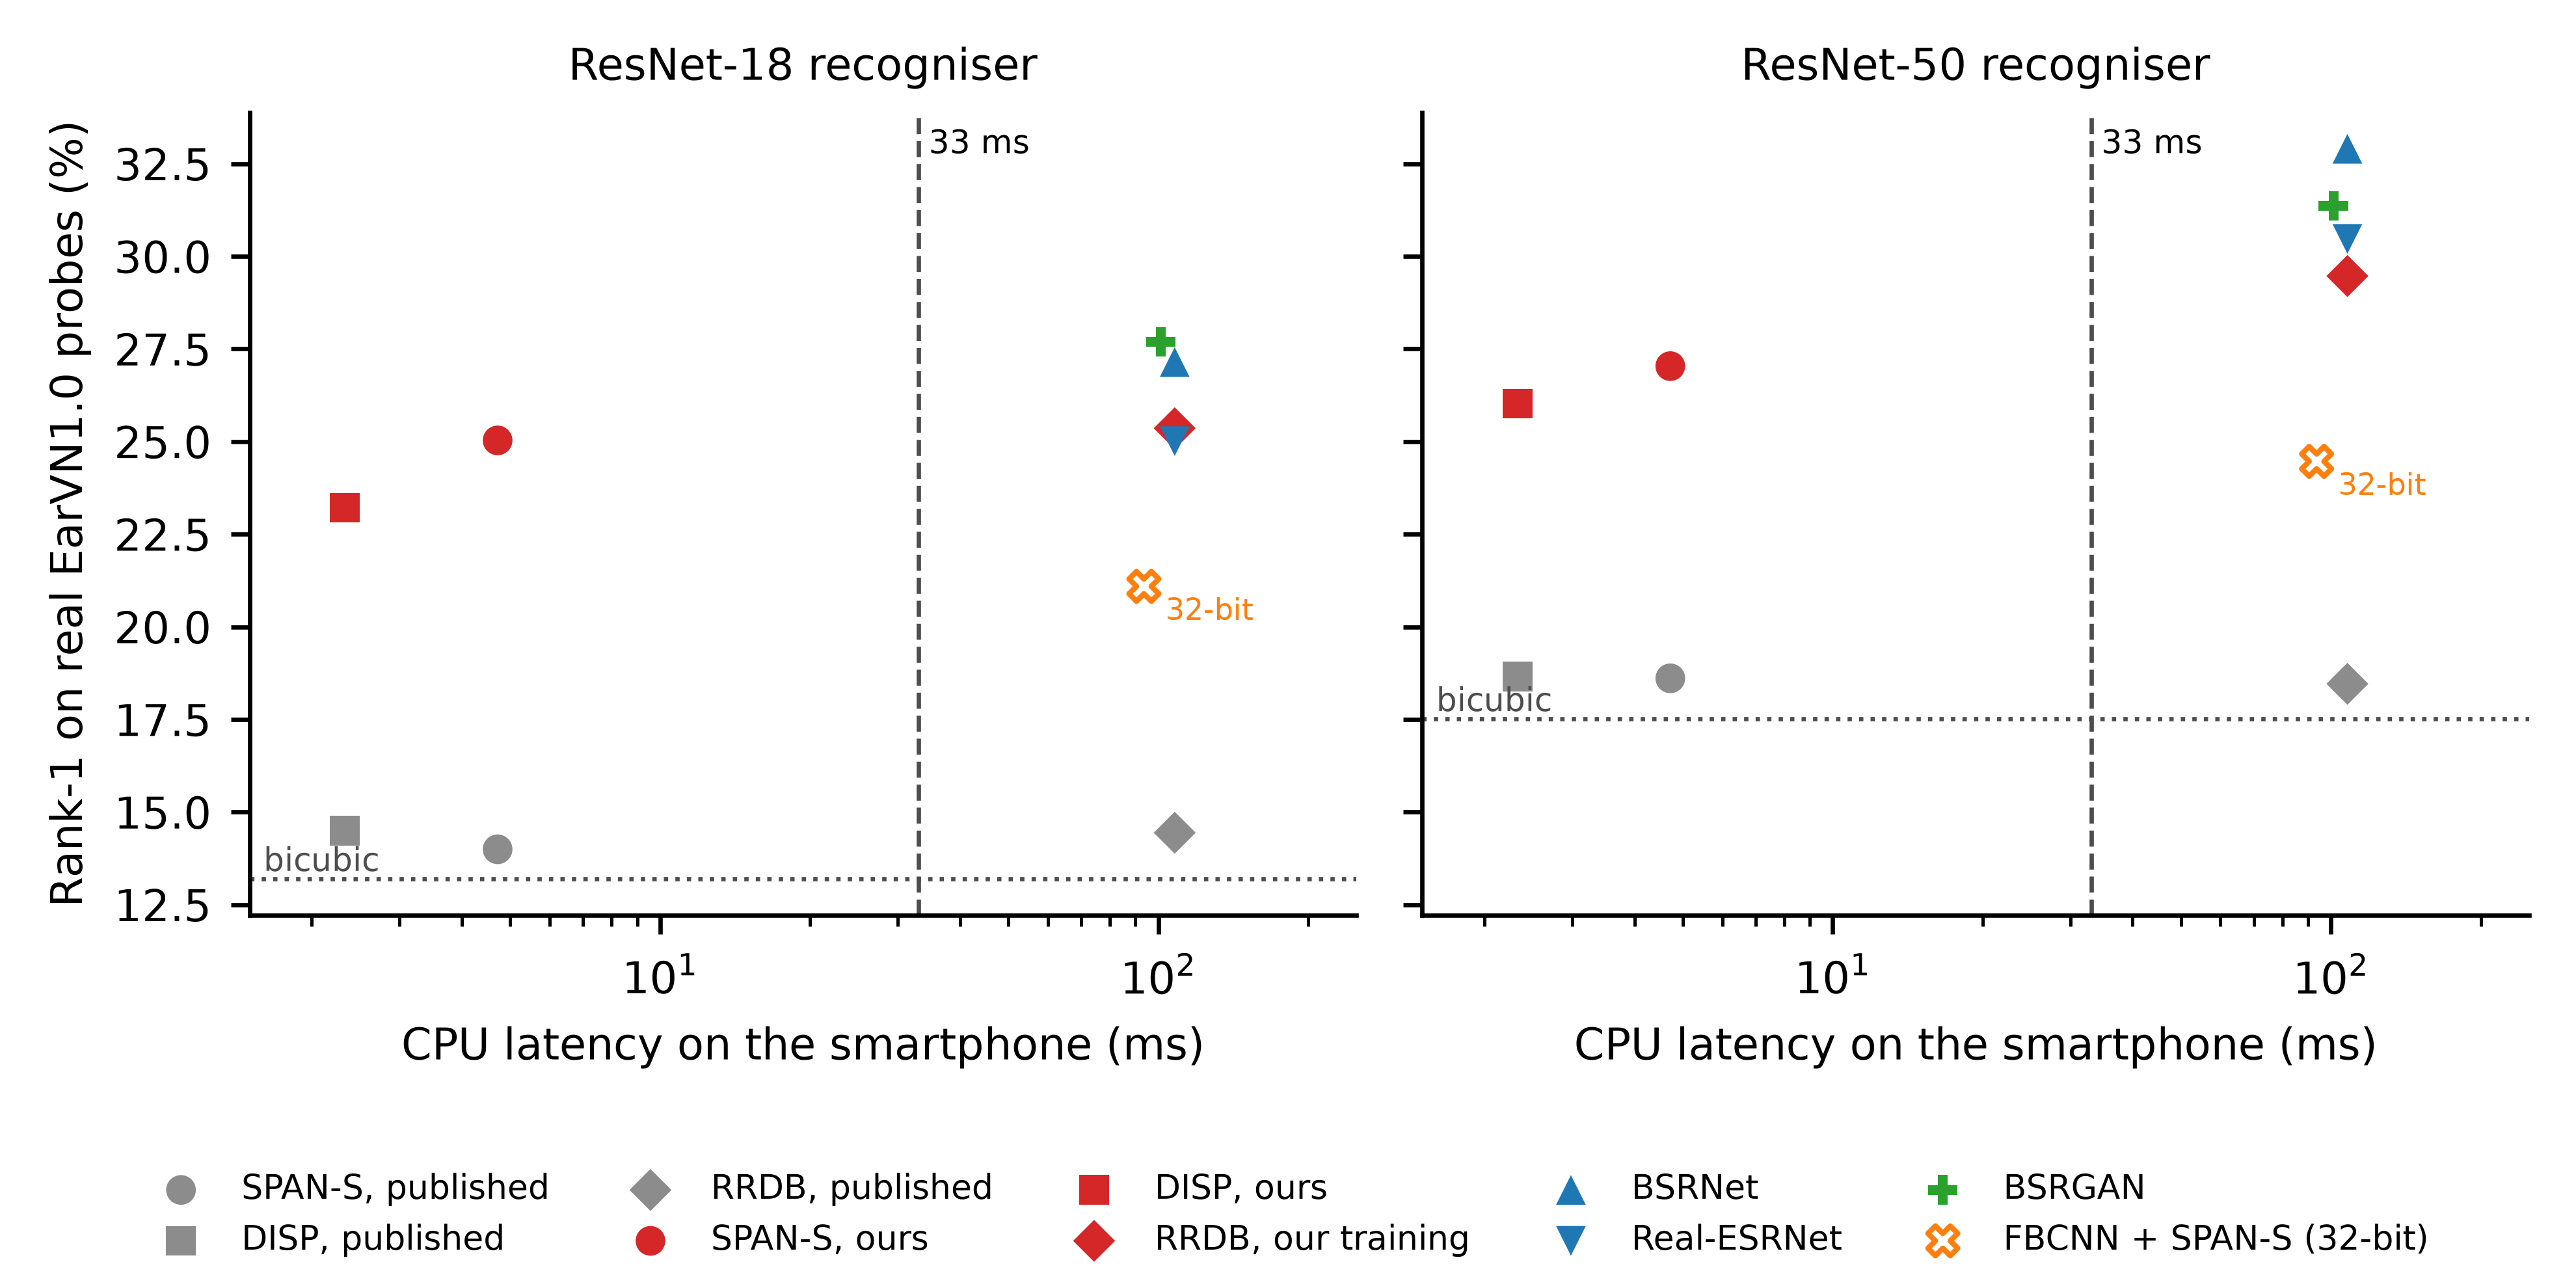
\includegraphics[width=\linewidth]{figures/fig_tradeoff.png}
\caption{Rank-1 rate on real EarVN1.0 probes against CPU latency on the \PhoneName{} for one $48\times68$ input. Dashed: real-time threshold; dotted: bicubic upscaling. BSRNet, Real-ESRNet and the fine-tuned RRDB share the measured latency of the RRDB architecture; FBCNN followed by SPAN (open marker) is measured in 32-bit precision, the other models in 16-bit precision.}
\label{fig:tradeoff}
\end{figure}

\section{Headroom of individual subjects}
\label{app:headroom}
We split the subjects at the median headroom (Section~\ref{sec:discussion}). Among the \HeadEarvnReSubj{} EarVN1.0 subjects with at least five small probes, the half with less headroom improves by \HeadEarvnReLowGain{} points and the half with more by \HeadEarvnReHighGain{} points with Ear-R18 (\HeadEarvnRfLowGain{} and \HeadEarvnRfHighGain{} with Ear-R50); the rank correlation between headroom and improvement is not significant (Spearman $\rho=\HeadEarvnReRho$, $p=\HeadEarvnReP$, and $\rho=\HeadEarvnRfRho$, $p=\HeadEarvnRfP$).

\section{Fidelity and identification}
\label{app:fidrecog}
Across the \CorrNAll{} methods, the rank-1 rate on real EarVN1.0 probes follows LPIPS on synthesised inputs and not PSNR (Table~\ref{tab:fidrecog}); without the two GAN-trained models, PSNR is also related to identification. The analysis was made after the identification results were known and describes this dataset only.

\begin{table}[H]
\centering
\caption{Spearman correlation between fidelity on synthesised EarVN1.0 inputs (measured degradation, 24-pixel inputs) and the rank-1 rate on real EarVN1.0 probes, across upscaling methods ($p$-values in parentheses). Negative values for LPIPS and DISTS mean that a lower distance goes with a higher rank-1 rate.}
\label{tab:fidrecog}
\fitbox{%
\begin{tabular}{@{}lrcccccc@{}}
\toprule
 & & \multicolumn{2}{c}{PSNR} & \multicolumn{2}{c}{LPIPS} & \multicolumn{2}{c}{DISTS} \\
\cmidrule(lr){3-4}\cmidrule(lr){5-6}\cmidrule(l){7-8}
Methods & $n$ & Ear-R18 & Ear-R50 & Ear-R18 & Ear-R50 & Ear-R18 & Ear-R50 \\
\midrule
\tabinput{generated/tab_fidrecog}
\bottomrule
\end{tabular}}
\end{table}

\section{Precision of the converted FBCNN}
\label{app:coreml}
The 16-bit Core ML conversion of FBCNN does not reproduce its output (PSNR \CoremlPsnrFbHalf{}~dB between Core ML and PyTorch outputs, against more than 50~dB for the other models), so FBCNN and, for comparison, SPAN are measured in 32-bit precision, where Core ML runs them on the GPU.
